% proci.tex

\cleardoublepage
\chapter{LODESTAR}\label{chapter:experimental-results}	

The program LODESTAR (Launch Optimisation and Data Evaluation for Scramjet Trajectory Analysis Research) has been developed to aid with the simulation and trajectory optimisation of space launch systems. LODESTAR is a MATLAB based trajectory optimiser which utilises GPOPS-2, a proprietary pseudospectral method optimisation package as well as MATLAB's inbuilt SQP solver. LODESTAR optimises a trajectory towards a user-defined objective function, such as constant dynamic pressure or maximum payload-to-orbit.  LODESTAR accurately models both rocket-powered and scramjet-powered vehicles in 5 degrees of freedom. LODESTAR contains multiple modules configured for the SPARTAN launch system, which are able to optimise trajectories for;
\begin{enumerate}
 \item The ascent of the first stage rocket.
 \item The ascent of the second stage scramjet-powered accelerator.
 \item The flyback of the second stage scramjet-powered accelerator.
 \item The ascent of the third stage rocket.
\end{enumerate}

\section{Optimal Control}
-background of general optimal control? 


The pseudospectral method and direct single shooting techniques used by LODESTAR are described in detail in sections X-X. Practically, the implementation of these techniques involves the specification of the set of constraints and objectives which govern the optimisation problem. These constraints inform the optimiser of the limits of the optimisation, and perform the functions of bounding the logical search space (eg. constraining altitude to be greater than ground level) as well as constraining the vehicle within its performance limits (eg. limiting the angle of attack). These constraints also come in the form of initial or terminal constraints, which define the initial conditions of the trajectory as well as any conditions which the trajectory must meet at termination. 

The pseudospectral method requires the specification of a set of 'primal variables'. These primal variables describe the physical dynamics of the system. In the pseudospectral method, the dynamics of the system are used as constraints on the optimal control problem;
\begin{equation} \label{eq:state2}
\dot{\textbf{x}}(\tau) = f[\textbf{x}(\tau),\textbf{u}(\tau)].
\end{equation}
Implementing the dynamics as constraints allows the optimiser to explore each primal variable independently, greatly increasing the robustness of the optimal control problem. However, the constraints may be violated by the optimiser in the process of searching for an optimal solution. A violation of the physical dynamics constraints means that the dynamics of the system may not hold throughout the solution process, causing potential complications for the computational model of the vehicle. Much of the design of the vehicle simulation in this study is driven by the need for smooth, continuous interpolation schemes, and viable extrapolation regions ie. even if the solution is well within the range of all input data sets, the solver must be able to explore all regions within the set bounds. 

\subsection{GPOPS-2 Example - Brachistochrone Problem}

-Maybe have analytical solution here?

The brachistochrone (from the Greek for 'shortest time') problem is a simple optimal control problem, which describes a ball rolling in two dimensions under gravity. The objective is to find the curve of descent which will minimise the time from point \textit{a}, where the ball is at rest, to point \textit{b}. It is assumed that gravity is constant and that there is no forces other than gravity acting on the ball. 

The analytical solution of this problem can be computed using the Euler-Lagrange equation as the equations describing a cycloid:

$x = A(\theta - \sin\theta) $,

$y=A(1 - \cos\theta)$

This problem has been solved using GPOPS-2. Table XX describes the set-up of the optimal control problem in GPOPS-2. 

\begin{tabular}{|c|c|}
	\hline Primal Variables  & x Position\\& y Position\\& Velocity\\ 
	\hline Control Variables  & Angle of Descent\\ 
	\hline Initial Constraints  & Velocity\\ & x Position\\ & y Position\\
	\hline Terminal Constraints &  x Position\\ & y Position\\
	\hline Path Constraints & None \\ 
	\hline Target Cost & Minimum Time \\ 
	\hline 
\end{tabular} 

The dynamic equations for the Brachistochrone problem are:

$\dot{x} = v*cos(u)$,

$\dot{y} = v*sin(u)$,

$\dot{v} = -g*sin(u)$.

The GPOPS-2 solution to the Brachistochrone problem is shown in Figure XX. This is overlaid with a plot of the optimal solution.

- xx put optimal solution in here 

The dynamics of the basic Brachistochrone problem are very simple. As the dynamic become more complex, it is no longer possible to obtain an analytical solution. 

\section{The Trajectory Optimal Control Problems}

\subsection{Dynamic Model}

 \textcolor{red}{images here.}
 - image detailing the coordinate system?
 - image detailing the point mass of the aircraft along with angle of attack / bank angle

The drag and lift produced by each stage of the vehicle are calculated using the standard definition of the aerodynamic coefficients:

\begin{equation}
F_d = \frac{1}{2}\rho c_d v^2 A ,
\end{equation}
\begin{equation}
F_L = \frac{1}{2}\rho c_L v^2 A .
\end{equation}

The dynamics of the vehicle are calculated in six degrees of freedom, with pitch constrained to zero. 
The dynamics of all stages are calculated using an geodetic rotational reference frame, written in terms of the angle of attack $\alpha$, bank angle $\eta$, radius from centre of Earth $r$, longitude $\xi$, latitude $\phi$, flight path angle $\gamma$, velocity $v$ and heading angle $\zeta$. The equations of motion are \cite{Josselyn2002a}:
\begin{figure}
\centering
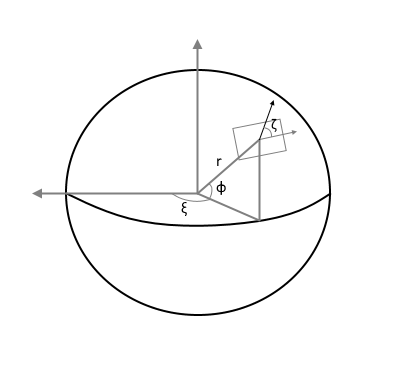
\includegraphics[width=0.7\linewidth]{figures/4_LODESTAR/global}
\caption{}
\label{fig:global}
\end{figure}
\begin{figure}
\centering
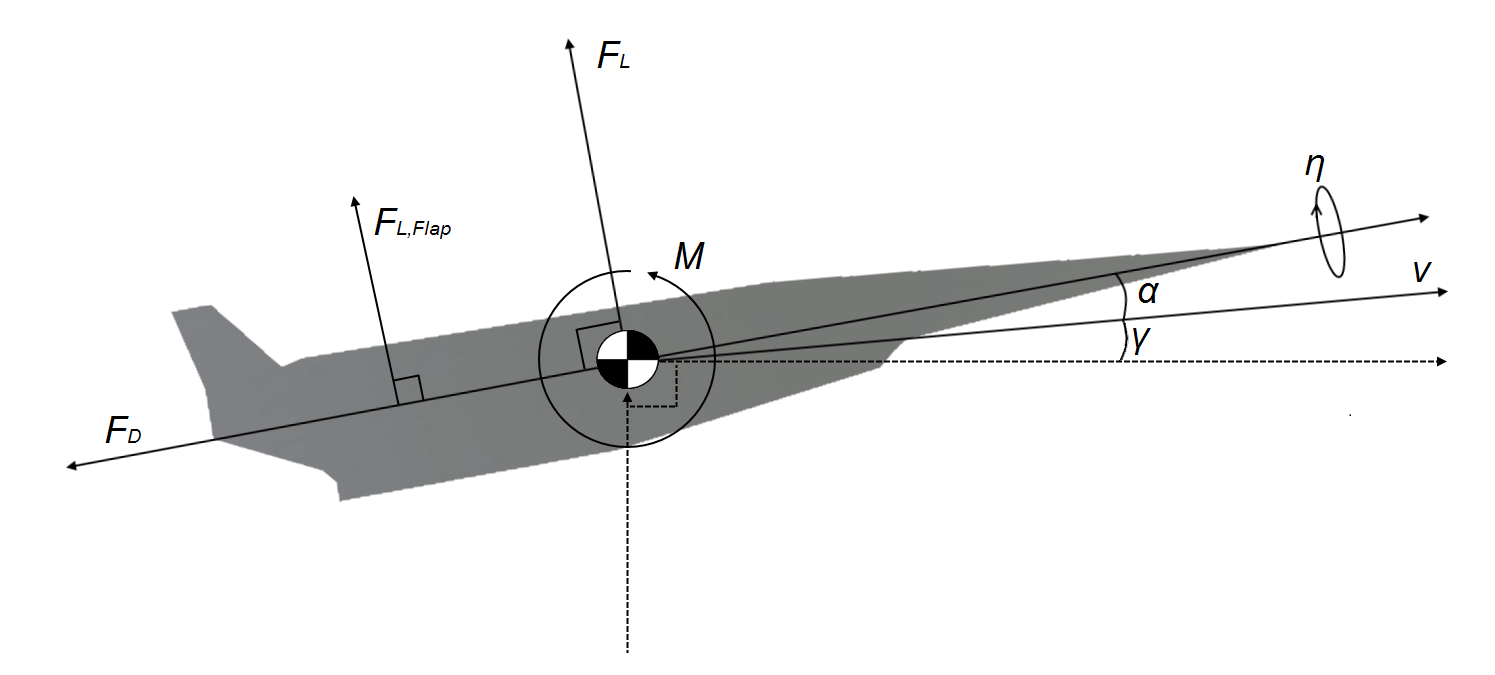
\includegraphics[width=0.9\linewidth]{figures/4_LODESTAR/Axes}
\caption{}
\label{fig:Axes}
\end{figure}


\begin{equation}
\dot{r} = v \sin \gamma
\end{equation}

\begin{equation}
\dot{\xi} = \frac{v\cos \gamma \cos \zeta}{r \cos \phi}
\end{equation}

\begin{equation}
\dot{\phi} = \frac{v\cos\gamma\sin\zeta}{r}
\end{equation}
\begin{equation}
\dot{\gamma} = \frac{T\sin\alpha \cos\eta}{mv} + (\frac{v}{r}-\frac{\mu_E}{r^2 v})\cos\gamma + \frac{L}{mv}
+ \cos\phi[2\omega_E \cos\zeta + \frac{\omega_E^2 r}{v}(\cos\phi\cos\gamma+\sin\phi\sin\gamma\sin\zeta)]
\end{equation}
\begin{equation}
\dot{v} = \frac{T\cos\alpha}{m}-\frac{\mu_E}{r^2}\sin\gamma - \frac{D}{m}
+ \omega_E^2 r\cos\phi(\cos\phi\sin\gamma-\sin\phi\cos\gamma\sin\zeta)
\end{equation}
\begin{equation}
\dot{\zeta} = \frac{T\sin\alpha \sin\eta}{mv}-\frac{v}{r}\tan\phi\cos\gamma\cos\zeta +2\omega_E\cos\phi\tan\gamma\sin\zeta - \frac{\omega_E^2 r}{v\cos\gamma}\sin\phi\cos\phi\cos\zeta-2\omega_E\sin\phi 
\end{equation}



	Flow chart of modules
	details of simulation (5DOF geodetic rotational)
	details of limits
	
	verification methods
	-hamiltonian/costates
	-complementary conditions
	-forward sim (for sanity checking, will need to detail deficiencies in this)
	-forward integration
	-logic check (ie solver is still a heuristic process, run multiple times with varying guess. Is solution logical?)

-Geodetic rotational coordinates 
-put coordinate system here
-Pontani has a typo is his paper remember
-add in portion of lift going towards changing heading angle due to roll. This is just simple centripetal force. 
$F=mr\omega^2$ $v=\omega r$



- outline the pseudospectral method, as implemented in GPOPS? ie with stage definitions

\subsection{Trajectory Connection Points}

The optimisation of a large, nonlinear system is a complex and time-consuming task. The optimisation of the trajectory of the rocket-scramjet-rocket launch system considered in this study is an extremely complex problem, if simulated in its entirety. It is a potentially unmanageable task to produce an optimised trajectory by considering the entire launch trajectory as a single nonlinear programming problem. 
To mitigate the complexity of the simulation, the trajectory of the rocket-scramjet-rocket launch system has been broken down into subsections, shown in Figure \ref{fig:Traj}. These contiguous subsections are then able to be analysed and optimised independently. The subsections of the trajectory are connected through the use of initial and end constraints on the independent optimisation problems. These constraints are described in Table \ref{tab:constraints}.

\begin{table}


\begin{tabularx}{\linewidth}{|X|X|X|}
	\hline \textbf{Section} & Initial Constraint & End Constraint  \\ 
	\hline $1^{st}$ Stage Vertical Ascent (\textcolor{red}{\rom{1}}-\textcolor{red}{\rom{2}}) & Constrained to start at a velocity of 0m/s. & Constrained to fly to 90m altitude and 30m/s velocity. \\ 
	\hline $1^{st}$ Stage Pitching Ascent (\textcolor{red}{\rom{2}}-\textcolor{red}{\rom{3}}) & Constrained to start at 90m altitude and 30m/s velocity & Constrained entirely to $2^{nd}$ stage initial conditions \\ 
	\hline $2^{nd}$ Stage Ascent (\textcolor{red}{\rom{3}}-\textcolor{red}{\rom{4}}) & Constrained to 1520m/s velocity. & Constrained to 102.0$^\circ$ heading angle, the approximate angle which allows the third stage to reach sun synchronous orbit.\\ 
	\hline $2^{nd}$ Stage Return (\textcolor{red}{\rom{4}}-\textcolor{red}{\rom{6}}) & Constrained entirely to $2^{nd}$ stage ascent end conditions. & Constrained to conditions approaching landing at the initial launch site. \\ 
	\hline $3^{rd}$ Stage Ascent (\textcolor{red}{\rom{4}}-\textcolor{red}{\rom{5}}) & Constrained entirely to $2^{nd}$ stage ascent end conditions.  & Flight parallel with Earth's surface.  \\ 
	\hline $3^{rd}$ Stage Hohmann Transfer (\textcolor{red}{\rom{5}}) & Constrained entirely to $3^{rd}$ stage ascent end conditions. & Constrained to sun synchronoud orbit.  \\ 
	\hline 
	
\end{tabularx} 

\label{tab:constraints}
\caption{}
\end{table}

\begin{figure}
\centering
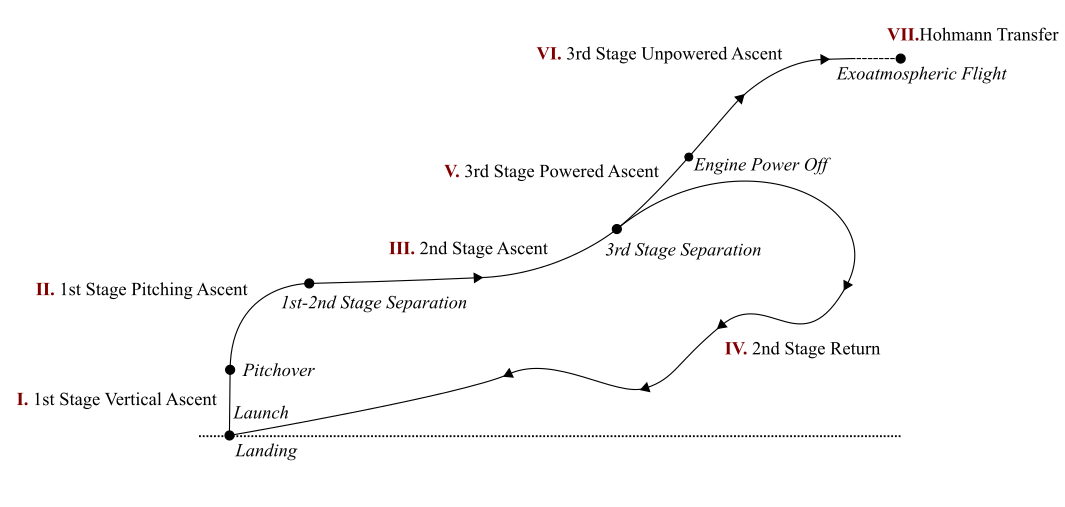
\includegraphics[width=1.\linewidth]{figures/4_LODESTAR/Traj}
\caption{}
\label{fig:Traj}
\end{figure}


\subsection{First Stage Trajectory}



LODESTAR is able to optimise the first stage of a launch vehicle, for an angle of attack controlled trajectory, from launch to a pre-defined end point. 
LODESTAR is able to optimise for either a maximum velocity or minimum mass optimisation objective. 

A maximum velocity case is desired when a specific first stage vehicle design is being investigated. 
 
A minimum mass objective is applicable when the first stage trajectory has a pre-defined end goal. This is the case with the SPARTAN vehicle where the SPARTAN scramjet accelerator is to be released at its minimum operating conditions at close to horizontal flight. 
A variable mass for the first stage launch vehicle is desired as the mass has large effects on the dynamics of th vehicle, effecting the trajectory angle change rate, as well as the acceleration and time of flight of the vehicle.
It is useful in the preliminary design stages to be able to optimise the mass of the first stage vehicle, allowing a less trial-and-error approach.
In the minimum mass case, the launch altitude is slightly variable, as LODESTAR starts optimisation from a set pitchover altitude and velocity, and the pre-pitchover trajectory is calculated to match the pitchover mass. 

\begin{tabular}{|c|c|}
	\hline Input  & Contains\\ 
	\hline Aerodynamic Database  & \\ 
	\hline 
\end{tabular} 


The first stage is launched from an area in northern Queensland.

\begin{tabular}{|c|c|}
	\hline Initial Constraints  & \\ 
	\hline Terminal Constraints &  \\ 
	\hline Path Constraints &  \\ 
	\hline Target Cost &  \\ 
	\hline 
\end{tabular} 

\subsubsection{Control Variables}

\subsubsection{Primal Variables}

\subsection{Second Stage Trajectory}

-detail the vehicle dynamics with a free body diagram 

LODESTAR is able to optimise the trajectory of airbreathing accelerators in the supersonic or hypersonic regime. LODESTAR is able to optimise for a range of optimisation metrics, including a maximum payload-to-orbit and constant dynamic pressure.  
The trajectory of the SPARTAN scramjet-powered accelerator has been simulated in LODESTAR. 

\begin{tabular}{|c|c|}
	\hline Initial Constraints  & Velocity \\ & Fuel Mass  \\ & Latitude \\ & Longitude \\ 
	\hline Terminal Constraints & Fuel mass \\ & Heading Angle \\ 
	\hline Path Constraints & Dynamic Pressure \\ 
	\hline Target Cost & Maximum Payload-to-Orbit \\ 
	\hline 
\end{tabular} 

\subsubsection{Control Variables}

\subsubsection{Primal Variables}
primal variable limits:

\subsection{Second Stage Return Trajectory}
After releasing the third stage rocket, the scramjet-powered second stage must return back to an area close to the initial launch site.
During the flyback, the SPARTAN cannot exceed its dynamic pressure limit of 50kPa. 
The SPARTAN must land on the ground with minimum velocity, within close proximity to the launch area. It is assumed that a landing strip is available at the spot where the SPARTAN lands. The SPARTAN is required to land within a set radius of the launch site. This constraint is;
\begin{equation}
(\phi_{end} - \phi_{launch})^2 + (\xi_{end} - \xi_{launch})^2 - r^2 \leq 0
\end{equation}



Summary Table

\begin{tabular}{|c|c|}
	\hline Initial Constraints  & Altitude \\ & Velocity\\ & Flight Path Angle\\ & Heading Angle\\ & Latitude\\ & Longitude\\ 
	\hline Terminal Constraints &  Distance From Launch Site \\ 
	\hline Path Constraints & Dynamic Pressure \\ 
	\hline Target Cost & Minimum End Velocity \\ 
	\hline 
\end{tabular} 

\subsubsection{Control Variables}


\subsection{Third Stage Trajectory}

-detail the vehicle dynamics with a free body diagram 

\begin{tabular}{|c|c|}
	\hline Input  & Contains\\ 
	\hline Aerodynamic Database  & Mach Number, AoA, CA, CN, CD, CL, cP\\ 
	\hline 
\end{tabular} 

\begin{tabular}{|c|c|}
	\hline Output  & Contains\\ 
	\hline   & \\ 
	\hline 
\end{tabular} 

The third stage is required to deliver the payload into heliosynchronous orbit. The heliosynchronous orbit chosen is 566.89km. 

\begin{tabular}{|c|c|}
	\hline Initial Constraints  & \\ 
	\hline Terminal Constraints &  \\ 
	\hline Path Constraints & Angle of Attack \\ 
	\hline Target Cost &  \\ 
	\hline 
\end{tabular} 


-Detail the hohmann transfer

\subsubsection{Control Variables}

\subsection{Combined Second Stage Ascent \& Return  Trajectory}

\subsection{Validation}
\subsubsection{Optimality Conditions}
Hamiltonian = 0 because dH/dt = 0 (Hamiltonian does not depend explicitly on time) except at end due to final time being free.
Costates
Complementary conditions

To assess the quality of the optimisation problem solved using the pseudospectral method, 

-need to calculate hamiltonian using continuous function... dont know that I can do this with GPOPS. the costates are different to what I understand. might not have enough info. 

\subsubsection{Forward Simulations}
-both the control check and derivative check

The pseudospectral method considers the dynamics of the system as constraints on the optimal control problem, and solves across the entire trajectory simultaneously. This causes the physical system dynamics to have an associated margin of error, ie. $\dot{x} = f(x)$ will only hold to a certain degree of accuracy. For a well converged solution, this margin of error will be negligibly small, and the dynamics of the system will be consistent with realistic Newtonian dynamics. However, when the problem is not well converged, the dynamics of the system may have a large error. It is possible to make a preliminary check of the system dynamics using the XX (complementary conditions?). However, to be certain that the system is behaving as it should be, a full forward simulation is necessary. This forward simulation starts at the initial conditions prescribed by the pseudospectral method solver, and propagates the dynamics of the system forward in time using numerical approximation. The forward simulation uses only inputs of the control sequence, as solved for by the pseudospectral method. 
